\chapter{Experimental details for HybridNet}
\label{chapter:hybridnetA}

\ifthenelse{\boolean{skipHN}}{\endinput}{}

\minitoc
\chapterwithfigures{\nameref*{chapter:hybridnetA}}
\chapterwithtables{\nameref*{chapter:hybridnetA}}

\section{Additional visualizations of HybridNet}

Additional visualizations of HybridNet behavior are presented in \autoref{hybridnetA:fig:cifar10} for CIFAR-10 and \autoref{hybridnetA:fig:stl10} for STL-10.

\newpage
\subsection{Additional results on CIFAR-10}

\begin{figure}[h]
	\centering
    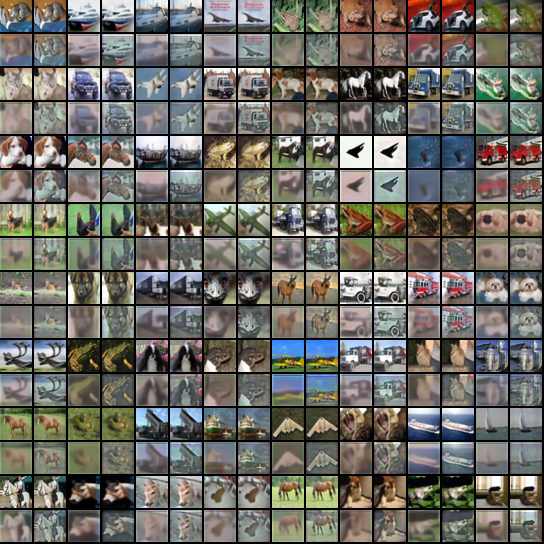
\includegraphics[width=\textwidth]{images/hybridnet_cifar10}
    \titlecaption{Example of visualizations for a ConvLarge-based HybridNet on CIFAR-10}{For each input image, there is block of 4 images on the figure with the following organization: $\begin{bmatrix}\vx&\vxh\\\vxh_c&\vxh_u\end{bmatrix}$.}
    \label{hybridnetA:fig:cifar10}
\end{figure}

\clearpage
\subsection{Additional results on STL-10}

\begin{figure}[h]
	\centering
    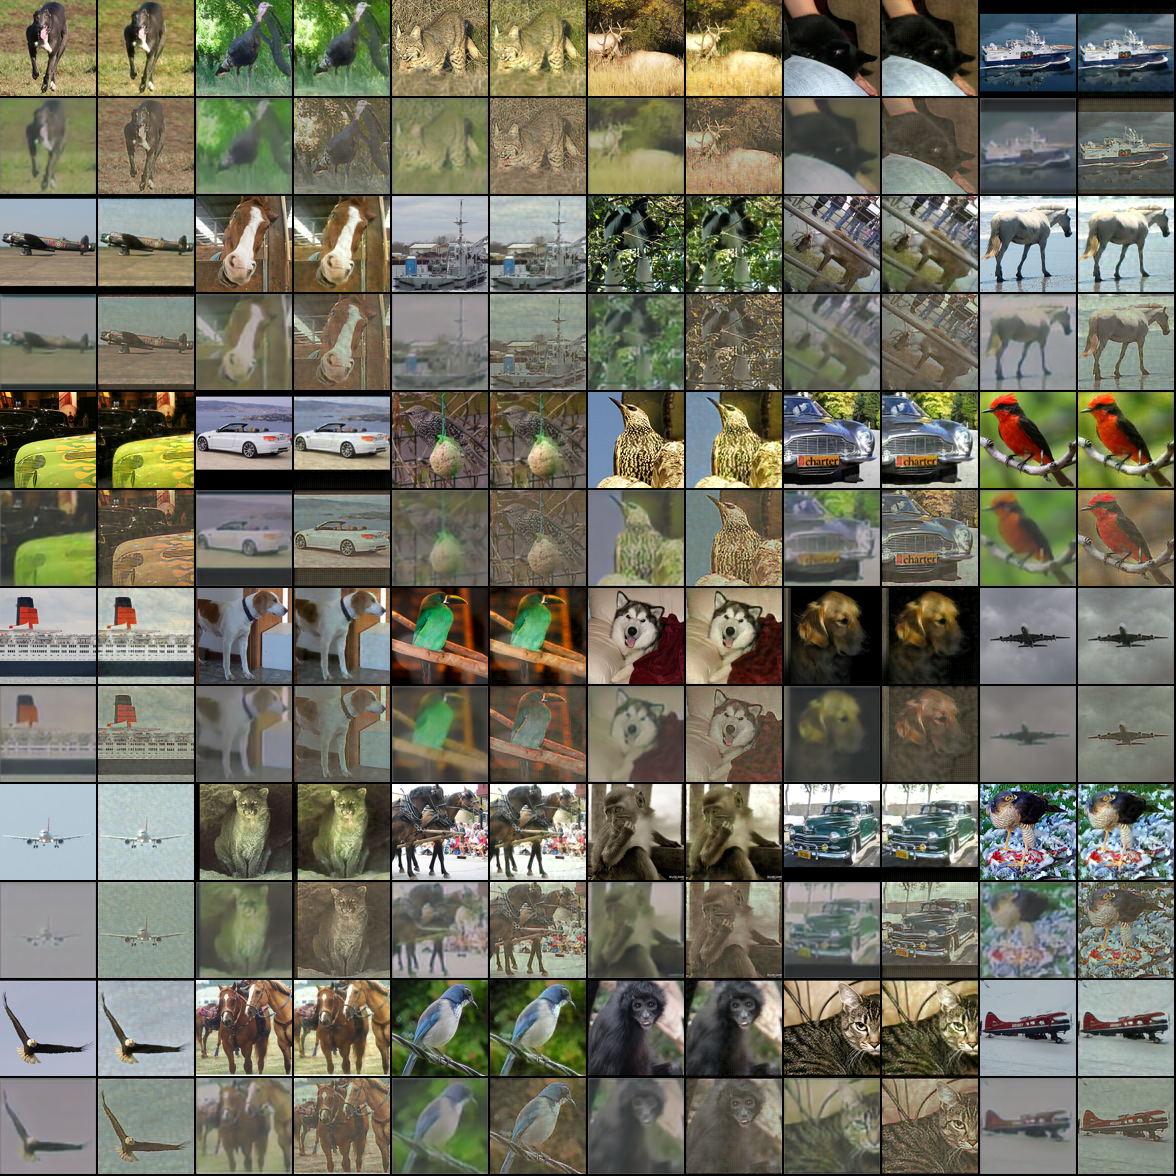
\includegraphics[width=\textwidth]{images/hybridnet_stl10}
    \titlecaption{Example of visualizations for a ConvLarge-like-based HybridNet on STL-10}{For each input image, there is block of 4 images on the figure with the following organization: $\begin{bmatrix}\vx&\vxh\\\vxh_c&\vxh_u\end{bmatrix}$.}
    \label{hybridnetA:fig:stl10}
\end{figure}

\FloatBarrier

\section{Experiment details}

\subsection{Experimental setup for ConvLarge on CIFAR-10}
\subsubsection{Data preprocessing and model architecture}

Input images are data-augmented with a random translation of a maximum of 2 pixels with mirror padding to fill-in the missing pixels, and randomly flipped. This constitutes the input $\vx$. We also add a Gaussian noise on $\vx$ $(\sigma=0.15)$ to obtain $\tilde\vx$ that is fed into the model.
The model's architecture is described in \autoref{hybridnetA:table:convlarge}.

\subsubsection{Training details}

The training method is similar to the one presented in recent paper using Conv\-Large \citep{Sajjadi2016,Laine2016,Tarvainen2017}.

The model is optimized with Adam during 60,000 batches (which corresponds to various number of epochs depending on the number of labeled images), with batches of 80 unlabeled samples and 20 labeled samples.

The weights of the various loss terms and the optimizer's parameters have base values and are varied over the training similarly to previous work using this model. The parameters' values and variations are summarized in \autoref{hybridnetA:table:convlargesched}. For the ablation study, parts of the model are removed and/or some weights are set to 0.


\subsection{Experimental setup for ConvLarge-like on STL-10}
\subsubsection{Model architecture}

Input images are data-augmented with a random translation of a maximum of 12 pixels with mirror padding to fill-in the missing pixels, and randomly flipped. This constitutes the input $\vx$. We also add a Gaussian noise on $\vx$ $(\sigma=0.15)$ to obtain $\tilde\vx$ that is fed into the model.
The model's architecture is detailed in \autoref{hybridnetA:table:convlargestl}.



\subsubsection{Training details}

The model is optimized with Adam during 150,000 batches (corresponding to 300 epochs over the labeled images, 48 epochs over the unlabeled images), with batches of 30 unlabeled samples and 2 labeled samples.
Hyperparameters' values and scheduling over training are detailed in \autoref{hybridnetA:table:convlargestlsched}.


\subsection{Experimental setup for ResNet on CIFAR-10 and SVHN}

The experimental setup described below follows the one described by \citet{Tarvainen2017} for a fair comparison.

\subsubsection{Model architecture}

\begin{figure}[tb]
	\centering
    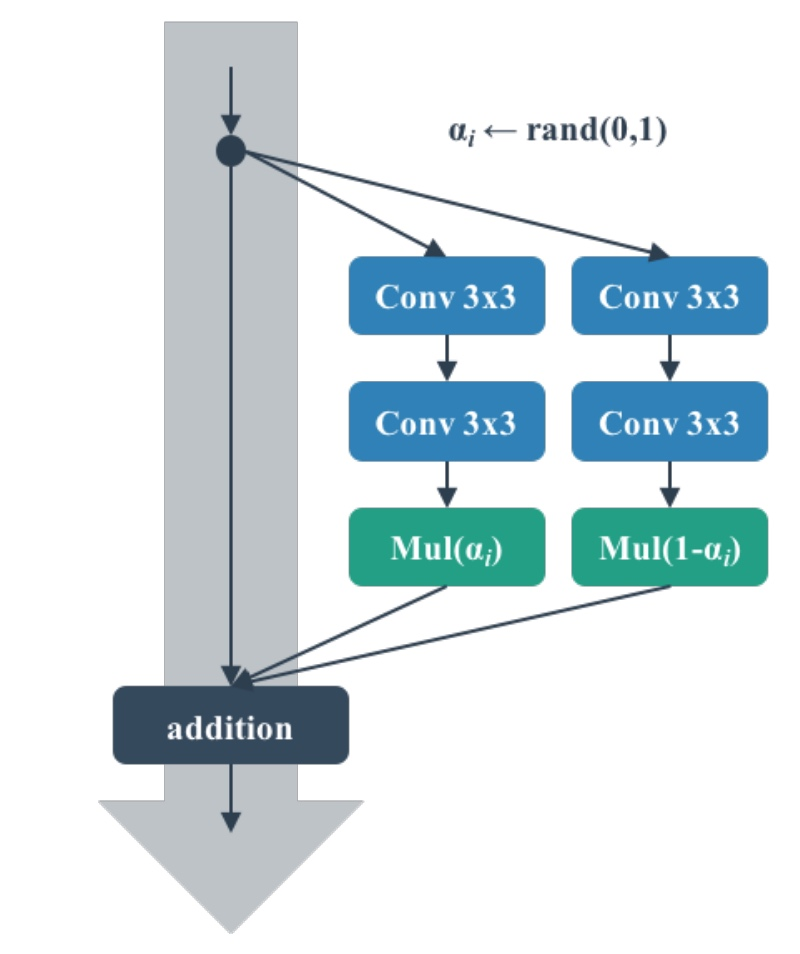
\includegraphics[width=0.45\textwidth]{images/hybridnet_shakeshake}
    \titlecaption{Shake-Shake building block}{}
    \label{hybridnetA:fig:shake}
\end{figure}

The data preprocessing simply consists in a classic per-color-channel mean-variance standardization. Images are data-augmented using random translation of a maximum of 4 pixels with mirror padding to fill-in the missing pixels and random flip. For SVHN, we disable image mirroring for obvious reasons.

We use the ResNet architecture with Shake-Shake building blocks described by \citet{Gastaldi2017}. A Shake-Shake building block consists of 2~similar branches each containing 2~convolutions, with the first one possibly having a stride greater that~1. The two branches are averaged with a weight $\alpha$ (see \autoref{hybridnetA:fig:shake} for illustration and the original paper for details) before being added to the result of a residual connection.

A ``layer'' is constituted of 4 blocks with possibly the first one having a stride in its first convolution and all convolutions having the same number of channels.

To reverse a layer, we apply the same strategy as before. This means that only the last transposed convolution of a decoding layer will have a smaller number of channels and a ``stride'' larger than~1 to reverse the first convolution of the corresponding layer in the encoder.

The architecture of the HybridNet based on this ResNet is described in \autoref{hybridnetA:table:resnet}.

\subsubsection{Training details for CIFAR-10}

The model's training is based on the settings of \citet{Tarvainen2017}. It is trained with Nesterov SGD with a base learning rate of 0.04 with a momentum of 0.9 over 300 epochs (one epoch correspond to one pass over the unlabeled images) with batches of 61 unlabeled images and 19 labeled images. Hyperparameters values and scheduling over training are detailed in \autoref{hybridnetA:table:resnetsched}.

\subsubsection{Training details for SVHN}

The model is trained with Nesterov SGD with a base learning rate of 0.04 with a momentum of 0.9 over 150 epochs (one epoch correspond to one pass over the unlabeled images) with batches of 265 unlabeled images and 15 labeled images. Hyperparameters values and scheduling over training are detailed in \autoref{hybridnetA:table:resnetschedsvhn} for SVHN.


\subsection{Experimental setup for ResNet on STL-10}

\subsubsection{Model architecture}

The model is a ResNet-50 pretraind on the Places dataset available at \url{https://github.com/CSAILVision/places365}. We did not use a model trained on ImageNet since the images of STL-10 have been extracted from ImageNet.

The data preprocessing simply consists in a classic per-color-channel mean-variance standardization. Images are data-augmented using random translation of a maximum of 30 pixels with mirror padding to fill-in the missing pixels and random flip.

\subsubsection{Training details}

The model is trained with Nesterov SGD with a base learning rate of 0.01 with a momentum of 0.9 over 350 epochs (one epoch correspond to one pass over the unlabeled images) with batches of 11 unlabeled images and 5 labeled images. Hyperparameters values and scheduling over training are detailed in \autoref{hybridnetA:table:resnetschedstl}.




\begin{table}[htbp]
\centering
\caption{Architecture of the HybridNet ConvLarge for CIFAR-10}
\label{hybridnetA:table:convlarge}
\begin{threeparttable}
\setlength{\tabcolsep}{4pt}
\begin{tabular}{ l l l}
\toprule
\multicolumn{3}{c}{\textbf{Encoders $E_c$ and $E_u$}} \\
\midrule
Input & $\tilde\vx$ & $32\times 32\times 3$ \\
Convolution & $128$ filters, $3\times3$, \textit{same} padding & $32\times 32\times 128$ \\
Convolution & $128$ filters, $3\times3$, \textit{same} padding & $32\times 32\times 128$ \\
Convolution & $128$ filters, $3\times3$, \textit{same} padding & $32\times 32\times 128$ \\
Pooling   & Maxpool $2\times2$ & $16\times 16\times 128$ \\
Dropout   & $p=0.5$  & $16\times 16\times 128$ \\
Convolution & $256$ filters, $3\times3$, \textit{same} padding  & $16\times 16\times 256$ \\
Convolution & $256$ filters, $3\times3$, \textit{same} padding  & $16\times 16\times 256$ \\
Convolution & $256$ filters, $3\times3$, \textit{same} padding  & $16\times 16\times 256$ \\
Pooling & Maxpool $2\times2$  & $8\times 8\times 256$ \\
Dropout & $p=0.5$  & $8\times 8\times 256$ \\
Convolution & $512$ filters, $3\times3$, \textit{valid} padding  & $6\times 6\times 512$ \\
Convolution & $256$ filters, $1\times1$, \textit{same} padding & $6\times 6\times 256$ \\
Convolution & $128$ filters, $1\times1$, \textit{same} padding & $6\times 6\times 128$ \\
Output & $\vh_c$ or $\vh_u$ & $6\times 6\times 128$ \\

\toprule
\multicolumn{3}{c}{\textbf{Classifier $C$}}\\
\midrule
Input & $\vh_c$& $6\times 6\times 128$ \\
Pooling & Global average pool & $1\times 1\times 128$ \\
Fully connected & with Softmax & $10$ \\
Output & $\vyh$ & 10 \\
\toprule
\multicolumn{3}{c}{\textbf{Decoders $D_c$ and $D_u$}}\\
\midrule
Input & $\vh_c$ or $\vh_u$ & $6\times 6\times 128$ \\
TConvolution & $256$ filters, $1\times1$, \textit{same} padding  & $6\times 6\times 256$ \\
TConvolution & $512$ filters, $1\times1$, \textit{same} padding  & $6\times 6\times 512$ \\
TConvolution & $256$ filters, $3\times3$, \textit{valid} padding  & $8\times 8\times 256$ \\
Upsampling   & $2\times2$ (unpooling in $D_u$)  & $16\times 16\times 256$ \\
TConvolution & $256$ filters, $3\times3$, \textit{same} padding & $16\times 16\times 256$ \\
TConvolution & $256$ filters, $3\times3$, \textit{same} padding & $16\times 16\times 256$ \\
TConvolution & $128$ filters, $3\times3$, \textit{same} padding & $16\times 16\times 128$ \\
Upsampling & $2\times2$ (unpooling in $D_u$) & $32\times 32\times 128$ \\
TConvolution & $128$ filters, $3\times3$, \textit{same} padding  & $32\times 32\times 128$ \\
TConvolution & $128$ filters, $3\times3$, \textit{same} padding  & $32\times 32\times 128$ \\
TConvolution & $3$ filters, $3\times3$, \textit{same} padding  & $32\times 32\times 3$ \\
Output & $\vxh_c$ or $\vxh_u$ & $32\times 32 \times 3$ \\
\bottomrule
\end{tabular}
\begin{tablenotes}
TConvolution stands for ``transposed convolution''.\\ Each Convolution or TConvolution is followed by a Batch Normalization layer and a LeakyRELU of parameter $\alpha = 0.1$
\end{tablenotes}
\end{threeparttable}
\end{table}


\begin{table}[htbp]
\centering
\caption{Evolution of weights for ConvLarge on CIFAR-10}
\label{hybridnetA:table:convlargesched}
\begin{threeparttable}
\setlength{\tabcolsep}{4pt}
\begin{tabular}{ l l l}
\toprule
& Value & Scheduling \\
\midrule
$\eta$ & 0.003 & Linear decrease to 0 over the last \nicefrac{1}{3} of the training \\
$\beta_1$ & 0.9 & Exponential decrease to 0.5 over the last \nicefrac{1}{5} of the training \\
$\lambda_c$ & 1 & Exponential increase from 0 over 800 first batches \\
$\lambda_s$ & 100 & Exponential increase from 0 over first \nicefrac{1}{4} of the training \\
& & and exponential decrease to 0 over the last \nicefrac{1}{5} of the training \\
$\lambda_r$ & 1 & Exponential decrease over the last 5\% of the training \\
\bottomrule
\end{tabular}
\begin{tablenotes}
$\eta$ is the learning rate, $\beta_1$ the first momentum of Adam, $\lambda_c$ the classification weight, $\lambda_s$ the stability weight, $\lambda_r$ the reconstructions weights.\\
Exponential decrease follows the function $\exp(-5t^2)$ with $t\in[0,1]$ from the start to the end of the decreasing interval. When increasing, $t$ goes from 1 to 0.
\end{tablenotes}
\end{threeparttable}
\end{table}





\begin{table}[htbp]
\centering
\caption{Architecture of the HybridNet ConvLarge-like architecture for STL-10}
\label{hybridnetA:table:convlargestl}
\begin{threeparttable}
\setlength{\tabcolsep}{4pt}
\begin{tabular}{ l l l}
\toprule
\multicolumn{3}{c}{\textbf{Encoders $E_c$ and $E_u$}} \\
\midrule
Input & $\tilde\vx$ & $96\times 96\times 3$ \\
Convolution & $64$ filters, $3\times3$, \textit{same} padding & $96\times 96\times 64$ \\
Convolution & $64$ filters, $3\times3$, \textit{same} padding & $96\times 96\times 64$ \\
Pooling   & Maxpool $2\times2$ & $48\times 48\times 64$ \\

Convolution & $128$ filters, $3\times3$, \textit{same} padding & $48\times 48\times 128$ \\
Convolution & $128$ filters, $3\times3$, \textit{same} padding & $48\times 48\times 128$ \\
Pooling   & Maxpool $2\times2$ & $24\times 24\times 128$ \\

Convolution & $256$ filters, $3\times3$, \textit{same} padding  & $24\times 24\times 256$ \\
Convolution & $256$ filters, $3\times3$, \textit{same} padding  & $24\times 24\times 256$ \\
Pooling   & Maxpool $2\times2$ & $12\times 12\times 256$ \\

Convolution & $256$ filters, $3\times3$, \textit{same} padding  & $12\times 12\times 256$ \\
Pooling & Maxpool $2\times2$  & $6\times 6\times 256$ \\

Output & $\vh_c$ or $\vh_u$ & $6\times 6\times 256$ \\

\toprule
\multicolumn{3}{c}{\textbf{Classifier $C$}}\\
\midrule
Input & $\vh_c$& $6\times 6\times 256$ \\

Convolution & $512$ filters, $4\times4$, \textit{valid} padding  & $3\times 3\times 512$ \\
Dropout & $p=0.5$  & $3\times 3\times 512$ \\
Convolution & $512$ filters, $1\times1$, \textit{same} padding & $3\times 3\times 512$ \\
Dropout & $p=0.5$  & $3\times 3\times 512$ \\
Convolution & $10$ filters, $1\times1$, \textit{same} padding & $3\times 3\times 10$ \\

Pooling & Global average pool & $1\times1\times10$ \\
Softmax &   & $10$ \\
Output & $\vyh$ & 10 \\
\toprule
\multicolumn{3}{c}{\textbf{Decoders $D_c$ and $D_u$}}\\
\midrule
Input & $\vh_c$ or $\vh_u$ & $6\times 6\times 256$ \\
Upsampling   & $2\times2$ (unpooling in $D_u$)  & $12\times 12\times 256$ \\
TConvolution & $256$ filters, $3\times3$, \textit{same} padding  & $12\times 12\times 256$ \\
Upsampling   & $2\times2$ (unpooling in $D_u$)  & $24\times 24\times 256$ \\
TConvolution & $256$ filters, $3\times3$, \textit{same} padding  & $24\times 24\times 256$ \\
TConvolution & $128$ filters, $3\times3$, \textit{same} padding  & $24\times 24\times 128$ \\
Upsampling   & $2\times2$ (unpooling in $D_u$)  & $48\times 48\times 128$ \\
TConvolution & $128$ filters, $3\times3$, \textit{same} padding  & $48\times 48\times 128$ \\
TConvolution & $64$ filters, $3\times3$, \textit{same} padding  & $48\times 48\times 64$ \\
Upsampling   & $2\times2$ (unpooling in $D_u$)  & $96\times 96\times 64$ \\
TConvolution & $64$ filters, $3\times3$, \textit{same} padding  & $96\times 96\times 64$ \\
TConvolution & $3$ filters, $3\times3$, \textit{same} padding  & $96\times 96\times 3$ \\
Output & $\vxh_c$ or $\vxh_u$ & $96\times 96 \times 3$ \\
\bottomrule
\end{tabular}
\begin{tablenotes}
TConvolution stands for ``transposed convolution''.\\ Each Convolution or TConvolution is followed by a Batch Normalization layer and a ELU activation.
\end{tablenotes}
\end{threeparttable}
\end{table}


\begin{table}[htbp]
\centering
\caption{Evolution of weights for ConvLarge-like on STL-10}
\label{hybridnetA:table:convlargestlsched}
\begin{threeparttable}
\setlength{\tabcolsep}{4pt}
\begin{tabular}{ l l l}
\toprule
& Value & Scheduling \\
\midrule
$\eta$ & 0.001 & Linear decrease to 0 over the last \nicefrac{1}{10} of the training \\
$\beta_1$ & 0.9 & Constant \\
$\lambda_c$ & 1 & Exponential increase from 0 over 4000 first batches \\
$\lambda_s$ & 300 & Exponential increase from 0 over first \nicefrac{1}{4} of the training \\
& & and exponential decrease to 0 over the last \nicefrac{1}{4} of the training \\
$\lambda_r$ & 1 & Exponential decrease over the last 5\% of the training \\
\bottomrule
\end{tabular}
\begin{tablenotes}
$\eta$ is the learning rate, $\beta_1$ the first momentum of Adam, $\lambda_c$ the classification weight, $\lambda_s$ the stability weight, $\lambda_r$ the reconstructions weights.\\
Exponential decrease follows the function $\exp(-5t^2)$ with $t\in[0,1]$ from the start to the end of the decreasing interval. When increasing, $t$ goes from 1 to 0.
\end{tablenotes}
\end{threeparttable}
\end{table}







\begin{table}[htbp]
\centering
\caption{Architecture of the HybridNet ResNet architecture for CIFAR-10 and SVHN}
\label{hybridnetA:table:resnet}
\begin{threeparttable}
\setlength{\tabcolsep}{4pt}
\begin{tabular}{ l l l}
\toprule
\multicolumn{3}{c}{\textbf{Encoders $E_c$ and $E_u$}} \\
\midrule
Input & $\tilde\vx$ & $32\times 32\times 3$ \\
Convolution & $16$ filters, $3\times3$, \textit{same} padding & $32\times 32\times 16$ \\

Shake Shake layer & $4$ blocks, $96$ filters, $3\times3$,  stride 1 & $32\times 32\times 96$ \\
Shake Shake layer & $4$ blocks, $192$ filters, $3\times3$,  stride 2 & $16\times 16\times 192$ \\
Shake Shake layer & $4$ blocks, $384$ filters, $3\times3$,  stride 2 & $8\times 8\times 384$ \\
Output & $\vh_c$ or $\vh_u$ & $8\times 8\times 384$ \\

\toprule
\multicolumn{3}{c}{\textbf{Classifier $C$}}\\
\midrule
Input & $\vh_c$& $8\times 8\times 384$ \\
Pooling & Global average pool & $1\times 1\times 384$ \\
Fully connected & with Softmax & $10$ \\
Output & $\vyh$ & 10 \\
\toprule
\multicolumn{3}{c}{\textbf{Decoders $D_c$ and $D_u$}}\\
\midrule
Input & $\vh_c$ or $\vh_u$ & $8\times 8\times 384$ \\
Shake Shake dec layer & $4$ blocks, $384$ filters, $3\times3$,  stride 2 & $8\times 8\times 192$ \\
Shake Shake dec layer & $4$ blocks, $192$ filters, $3\times3$,  stride 2 & $16\times 16\times 96$ \\
Shake Shake dec layer & $4$ blocks, $96$ filters, $3\times3$,  stride 1 & $32\times 32\times 16$ \\
Output & $\vxh_c$ or $\vxh_u$ & $32\times 32 \times 3$ \\
\bottomrule
\end{tabular}
\begin{tablenotes}
\end{tablenotes}
\end{threeparttable}
\end{table}

\begin{table}[htbp]
\centering
\caption{Evolution of weights for HybridNet ResNet architecture for CIFAR-10}
\label{hybridnetA:table:resnetsched}
\begin{threeparttable}
\setlength{\tabcolsep}{4pt}
\begin{tabular}{ l l l}
\toprule
    & Value & Scheduling \\
\midrule
$\eta$ & 0.04 & Cosine decrease over the full training \\
$\lambda_c$ & 1 & Constant \\
$\lambda_s$ & 300 & Constant \\
$\lambda_r$ & 0.25 & Exponential increase over the first 5 epochs \\
${\lambda_r}_{b,l}$ & 0.5 & Exponential increase over the first 2 epochs \\
\bottomrule
\end{tabular}
\begin{tablenotes}
$\eta$ is the learning rate, $\lambda_c$ the classification weight, $\lambda_s$ the stability weight, $\lambda_r$ the final reconstruction weight, ${\lambda_r}_{b,l}$ the intermediate reconstructions weights.\\
Exponential decrease follows the function $\exp(-5t^2)$ with $t\in[0,1]$ from the start to the end of the decreasing interval. When increasing, $t$ goes from 1 to 0.\\
Cosine decrease follows the function $\cos(\pi t)+1$ with $t\in[0,1]$ from the start to the end of the decreasing interval.
\end{tablenotes}
\end{threeparttable}
\end{table}



\begin{table}[htbp]
\centering
\caption{Evolution of weights for HybridNet ResNet architecture for SVHN}
\label{hybridnetA:table:resnetschedsvhn}
\begin{threeparttable}
\setlength{\tabcolsep}{4pt}
\begin{tabular}{ l l l}
\toprule
    & Value & Scheduling \\
\midrule
$\eta$ & 0.04 & Cosine decrease over the full training \\
$\lambda_c$ & 1 & Constant \\
$\lambda_s$ & 100 & Exponential increase over the first 5 epochs \\
$\lambda_r$ & 0.1 & Exponential increase over the first 5 epochs \\
${\lambda_r}_{b,l}$ & 0.2 & Exponential increase over the first 2 epochs \\
\bottomrule
\end{tabular}
\begin{tablenotes}
$\eta$ is the learning rate, $\lambda_c$ the classification weight, $\lambda_s$ the stability weight, $\lambda_r$ the final reconstruction weight, ${\lambda_r}_{b,l}$ the intermediate reconstructions weights.\\
Exponential decrease follows the function $\exp(-5t^2)$ with $t\in[0,1]$ from the start to the end of the decreasing interval. When increasing, $t$ goes from 1 to 0.\\
Cosine decrease follows the function $\cos(\pi t)+1$ with $t\in[0,1]$ from the start to the end of the decreasing interval.
\end{tablenotes}
\end{threeparttable}
\end{table}




\begin{table}[htbp]
\centering
\caption{Evolution of weights for HybridNet ResNet architecture for STL-10}
\label{hybridnetA:table:resnetschedstl}
\begin{threeparttable}
\setlength{\tabcolsep}{4pt}
\begin{tabular}{ l l l}
\toprule
    & Value & Scheduling \\
\midrule
$\eta$ & 0.01 & Exponential decrease during the last 8 epochs \\
$\beta_1$ & 0.9 & Exponential increase during the last 80 epochs down to 0.5 \\
$\lambda_c$ & 0.1 & Constant \\
$\lambda_s$ & 0.1 & Exponential increase over the first 150 epochs \\
$\lambda_r$ & 0.01 & Exponential decrease during the last 17 epochs \\
${\lambda_r}_{b,l}$ & 0.01 & Exponential decrease during the last 17 epochs \\
\bottomrule
\end{tabular}
\begin{tablenotes}
$\eta$ is the learning rate, $\beta_1$ the first momentum of Adam, $\lambda_c$ the classification weight, $\lambda_s$ the stability weight, $\lambda_r$ the final reconstruction weight, ${\lambda_r}_{b,l}$ the intermediate reconstructions weights.\\
Exponential decrease follows the function $\exp(-5t^2)$ with $t\in[0,1]$ from the start to the end of the decreasing interval. When increasing, $t$ goes from 1 to 0.\\
Cosine decrease follows the function $\cos(\pi t)+1$ with $t\in[0,1]$ from the start to the end of the decreasing interval.
\end{tablenotes}
\end{threeparttable}
\end{table}
